%-------------------------------------------------------------------------------------------------------------------------------------------------
\section{Fuzzy System}
%-------------------------------------------------------------------------------------------------------------------------------------------------
\label{sec:fuzzy}
Our third approach for SC is a bot which performs small-scale combats on a flat terrain. The objective of this combat is to annihilate the opponent's units and the same amount and the same types of units are fighting against each other.
The decision-making of a unit is based on a Fuzzy Inference System.
%IMPLEMENTATION
The Fuzzy-System got implemented by our selfs and uses a stack for representing rules. The implementation got inspired by an open source AI framework called {\tt AForge.NET}\footnote{\url{http://code.google.com/p/aforge/}}.  %CITE to AForge?
%CITE to Game Programming Gems and lecture notes/slides
Further inspiration on how to use and implement fuzzy systems can be found in \cite{gpuGems2_fuzzy} and in our lecture notes.

In order to develop a squad control we decided to make the logic individuall for each unit. In contrast to GA or QL the unit performs strategies that suit group combats. Each unit decides on a individual basis and can perform the following actions:
\begin{description}
	\item[Attack:] \hfill \\
A unit performing this action attacks the enemy unit, with the lowest hit points.
	\item[Retreat:] \hfill \\
A retreating unit is moving away from the centroid of all enemy units.
\end{description}
The strategy of attacking the weakest unit is known to be effective in SC and is called \emph{focus fire}\footnote{\url{http://starcraft.wikia.com/wiki/Focus_fire}}. %
Due to the fact that lesser units cannot cause as much damage, this strategy tries to always kill the weakest. With weakest unit we mean the unit with the least amount of remaining hit points. The weakest one is also supposed to die fast resulting in a reduced enemy squad and less units able to attack our units. 

Our fuzzy logic tries to tackle this strategy by using a prevention system, which moves units, in danger to die, from the front-line to the back of our squad.

%REPRESENATION
%
%%FIGURE WITH THE RULES
%%%
\begin{figure*}[htbp]
\begin{center}
\begin{tabular}{ccc}
{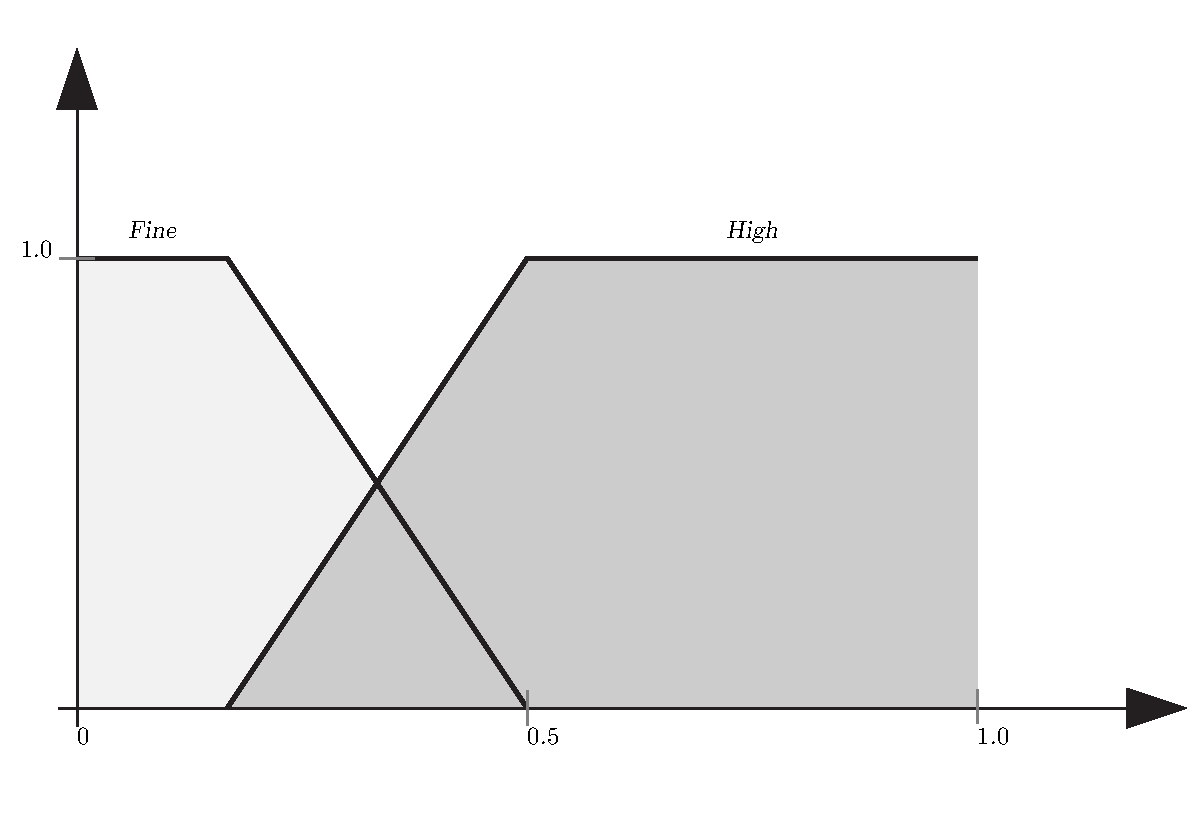
\includegraphics[width=1.0\columnwidth]{fig_fuzzy_deltaHealth}}&
{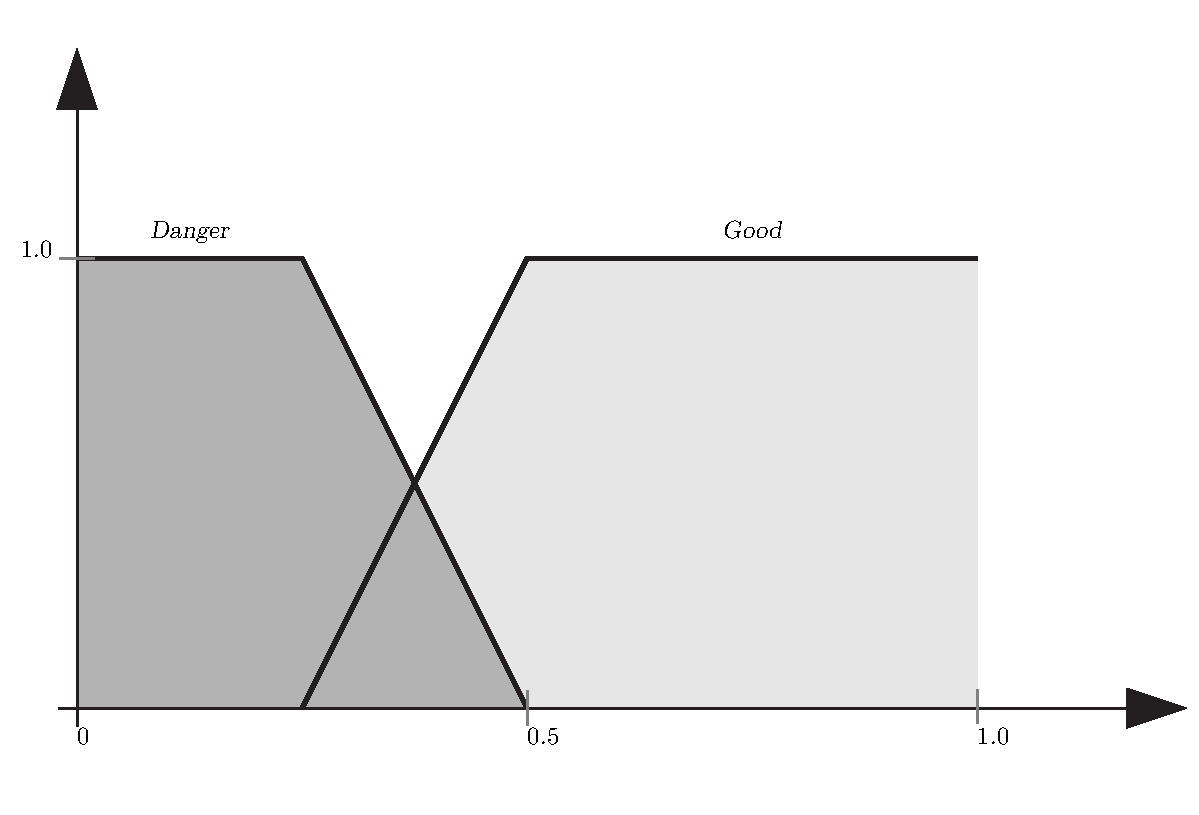
\includegraphics[width=1.0\columnwidth]{fig_fuzzy_health}}\\
{\it DeltaHealth } & {\it HitPoints }  \\
(a) & (b) \\
\end{tabular}
\end{center}
\caption{Linguistic variables and their fuzzy sets}
\label{fig:fuzzy_sets}
\end{figure*}
%
\begin{figure}
\begin{center}
\begin{tabular}{ccc}
{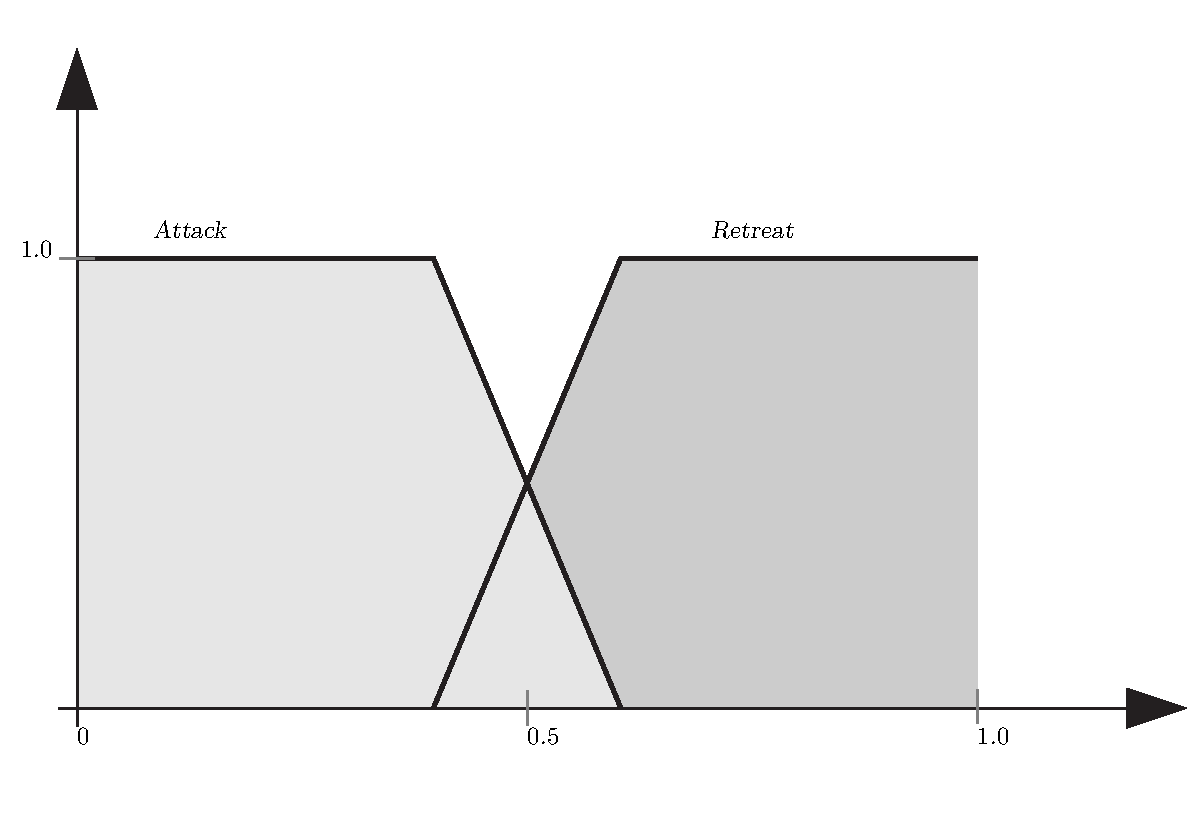
\includegraphics[width=1.0\columnwidth]{fig_fuzzy_stance}} \\ 
{\it Stance} \\
 (a) \\
\end{tabular}
\end{center}
\caption{Linguistic variable {\it Stance} and its fuzzy sets}
\label{fig:fuzzy_sets1}
\end{figure}
%%%
%%
%
For this approach we introduce three linguistic variables: {\it deltaHealth } ($\Delta \textrm{hP}$), {\it HitPoints } ($\textrm{hP}$) and {\it Stance}.
The fuzzy sets of the variables are as follows:
\begin{description}
	\item[{\it DeltaHealth:}] \hfill
	\begin{itemize}
		\item {\it Fine}
		\item {\it High}
	\end{itemize}
	\item[{\it HitPoints:}]  \hfill
	\begin{itemize}
		\item {\it Good}
		\item {\it Danger}
	\end{itemize}
	\item[{\it Stance:}]  \hfill
		\begin{itemize}
		\item {\it Attack}
		\item {\it Retreat}
	\end{itemize}
\end{description}

For a better overview the Figures \ref{fig:fuzzy_sets}(a), (b) and figure \ref{fig:fuzzy_sets1}(a) show the plotted fuzzy sets. The particular values of the fuzzy set get discussed later because we run some tests differing them. The range of all three variables is from $0.0$ to $1.0$. If a variable gets set above or below this range the values get clamped.

% Normalization of Inputs
Due to the fact that {\it DeltaHealth} only rises one frame, directly after we got hit by an enemy the impact of it would be only a short term one. To extend the range of one high hit, we calculate the {\it DeltaHealth} ($\Delta \textrm{hP}_i$) at a certain frame $i$ the following way:
\begin{align}
	\Delta \textrm{hP}_i &= \frac{( \textrm{hP}_{i-1} - \textrm{hP}_i ) + \Delta \textrm{hP}_{i-1}}{2}  \text{,}
\end{align}
where $\textrm{hP}_{i}$ is the {\it HitPoints} at the frame $i$. Before providing those values to the system they get normalized in the following way:
\begin{align}
	\textrm{inputDeltaHP}_i 	&= \frac{\Delta \textrm{hP}_i}{ \textrm{hP}_i} \\
 	\textrm{inputHP}_i 	&= \frac{\textrm{hP}_i}{ \textrm{maxHP}}  \text{,}
\end{align}
where $\textrm{inputDeltaHP}_i$, $\textrm{inputDeltaHP}_i$ are the inputs at frame $i$ and $ \textrm{maxHP}$ is the unit's initial amount of {\it HitPoints}.


With those fuzzy sets and variables we compose the following fuzzy rules:
\begin{enumerate}
	\item {\sl IF DeltaHealth IS High AND Health IS Danger THEN Stance IS Retreat }
	\item {\sl IF Health IS NOT Danger THEN Stance IS Attack }
\end{enumerate}

% :D ... fancy graph of the upper equations, maybe? :D

We applied our fuzzy set on different types of squad formations and we also differed the parameters for the fuzzy sets. Currently we only use the fuzzy sets {\it deltaHealth - High} and {\it HitPoints - Danger}. Due to that fact we don't talk about values for the other sets.
For our first test set, we call it \emph{fuzzy set 1}, we set {\it DeltaHealth - High} to the values $0.2$ and $0.5$. As shown in Figure \ref{fig:fuzzy_sets} this is a trapezoidal set which starts to rise from $0.2$ until it reaches the maximum at $0.5$ and stays at the maximum.
{\it HitPoints - Danger} got set to $0.3$ and $0.5$ which means the trapezoid starts with the maximum output at $0.0$ and falls in the range of $0.3$ to $0.5$ to a zero output.
Another test set (\emph{fuzzy set 2}) keeps the structure of  \emph{fuzzy set 1} and just moves the edges of the trapezoids.  {\it DeltaHealth - High} is  $0.00001$ and $0.1$ and {\it HitPoints - Danger} is set to $0.9$ and $0.99$.
\emph{Fuzzy set 3} sets {\it DeltaHealth - High} to $0.0001$ and $0.05$ and setting the fuzzy set {\it HitPoints - Danger} to $0.4$ and $0.5$.

The variable {\it Stance} stays the same for all tests and its fuzzy sets are trapezoidal shaped and are basically mirrored at the mid point ($0.5$). The {\it Attack} set covers the left half of the variable range with the values $0.4$ and $0.6$. {\it Retreat} also has the anchor points at $0.4$ and $0.6$, but this set covers the right half. Figure \ref{fig:fuzzy_sets1} (a) shows this set.

%LINGUISTIC VARIABLE AND IT'S MAPPING

%
\subsection{Results}
%-------------------------------------------------------------------------------------------------------------------------------------------------
%%%
\label{subsection:fuzzy:results}
%
Although the mechanics in SC are deterministic (especially weapon range and damage), the standard SC bot against whom our bot has to compete, makes random decisions. Therefore we have to run more games and average them. Most results in this section are the findings over a period of 100 games.
%
%%
\begin{table*}[htbp]
\caption{Fuzzy Logic: 2 Goliaths and 3 Marines Vs. 2 Goliaths and 3 Marines}
\begin{center}
\begin{tabular}{|l|r|c|c|c|c|c|c|c|ccccc}
\hline
	&  & \multicolumn{3}{|c|}{\bf summed HitPoints} 	& \multicolumn{3}{|c|}{\bf remaining units}  \\
	& \multicolumn{1}{|c|}{\bf lost} & $\mu$ & $\sigma$ & $p$ & 		$\mu$ & $\sigma$ & $p$ \\
\hline
{\it attacking (ref)}			&$ 1   $&$ 	176.12 $&$  48.52$&$ - $&$			2.63 $&$   0.87 $&$ - $ \\ %onlyAttacking.xlsx
\emph{ fuzzy set 1} 		&$ 2   $&$ 	153.61$&$   54.17$&$ 0.00 $&$ 			2.29 $&$   0.94 $&$ 0.00 $\\ %slighlyRetreating
\emph{ fuzzy set 2}		&$ 12 $&$ 	134.15 $&$  77.17$&$ 0.00 $&$     		2.15 $&$   1.13 $&$ 0.00 $ \\ %alwayRetreatingFuzzy.xlsx
\emph{ fuzzy set 3}		&$ 0 $&$ 	173.02 $&$  52.81$&$ 0.56 $&$     		2.59 $&$   0.85 $&$ 0.64 $ \\ %fuzzySet3.xlsx
%														not rejected at all
\hline
\end{tabular}  
\label{table:fuzzy_tTestSmallSquad}
\end{center}
\end{table*}
%%
%
Our initial tests with our three fuzzy set configurations are shown in Table \ref{table:fuzzy_tTestSmallSquad}. The squad for testing are 3 {\it marines} and 2 {\it goliaths} versus the same squad.
The table shows the average ($\mu$) and the standard deviation ($\sigma$) of the summed {\it HitPoints} and of our remaining units, for 100 games. The column \emph{lost} shows the amount of times the bot has lost out of this 100 games. As a reference we use a logic which is only attacking the weakest unit an never redrawing.
Initially there have been $5$ units and the initial sum of {\it HitPoints} is $370$.  The $p$-values can be found in the column $p$ and represent the results of a two-tailed test. 
%
%%
\begin{table*}[htbp]
\caption{Fuzzy Logic: 8 Goliaths Vs. 8 Goliaths}
\begin{center}
\begin{tabular}{|l|r|c|c|c|c|c|c|c|c|c|c|ccccc}
\hline
	&  & \multicolumn{3}{|c|}{\bf summed HitPoints} 	& \multicolumn{3}{|c|}{\bf remaining units}  &  \multicolumn{3}{|c|}{\bf frames per game}  \\
	& \multicolumn{1}{|c|}{\bf lost} & $\mu$ & $\sigma$ & $p$ & 		$\mu$ & $\sigma$ & $p$  & 	$\mu$ & $\sigma$ & $p$\\
\hline
{\it attacking (ref)}	&$ 1 $&$ 375.41 $&$   	126.88 $&$ - $&$			5.00 $&$   1.30 $&$ - $&$	 	415.61 $&$ 66.47  $&$ - $\\
\emph{ fuzzy set 3 }		&$ 4 $&$ 363.68 $&$    	152.92$&$ 0.44 $&$     		5.23 $&$   1.70 $&$ 0.18 $&$ 	427.54 $&$ 82.79 $&$ 0.15 $\\
\emph{ fuzzy set 3 (cleaned)} 	&$ 0 $&$ 380.30 $&$ 	136.29$&$ 0.72 $&$ 		5.48 $&$   1.36 $&$ 0.00  $&$ 	419.79 $&$ 76.11 $&$ 0.58 $\\
%								not rejected at all			rejected at 10 % significance level		rejected at 10% significance
%								not rejected at all			rejected at 1,5 and 10% significane level	not rejected at all
\hline
\end{tabular}  
\label{table:fuzzy_tTestBigSquad}
\end{center}
\end{table*}
%%
%
When this fuzzy logic gets applied to a different squad toplogy like eight {\it goliaths} versus eight {\it goliaths} it performs as shown in Table \ref{table:fuzzy_tTestBigSquad}. The table shows the average ($\mu$) and the standard deviation ($\sigma$) of the summed {\it HitPoints}, of our remaining units and the lost count of 100 games. The initial number of HitPoints when a game starts is $1000$ and there have been $8$ initial units. As a reference we use a simple logic which is only attacking the weakest unit an never redrawing. With a t-test we can show that some results are significantly better than the reference. The $p$-values can be found in Table \ref{table:fuzzy_tTestBigSquad} under the column $p$ and represent the results of a two-tailed test. 
The row {\it fuzzy set 3 (cleaned)} shows the data set when the $4$ lost games got removed.

%
\subsection{Discussion}
%-------------------------------------------------------------------------------------------------------------------------------------------------
%%%
The results of our test with the {\it marines} and {\it goliath} squad presented in Table \ref{table:fuzzy_tTestSmallSquad}, show that changing the fuzzy sets has an impact on the performance of our squad bot in the game. \emph{Fuzzy set 1} and \emph{ fuzzy set 2} are significantly worse than the simple attacking bot, in preserving HitPoints and in keeping units alive. The null hypothesis of the t-test gets rejected with a significance level of $1\%$.
The \emph{fuzzy set 3} bot seems better balanced and it cannot be shown that it is performing better or worse than the reference bot.
The bad performance of the \emph{ fuzzy set 2} bot can be explained by its behavior. It is retreating after every hit it takes and therefore gets more inefficient when the squad is decreasing, due to deaths of own units. The bot has no information about the squad-size and also withdraws even if there is only one unit left.
\emph{ Fuzzy set 1} is not as bad as \emph{ fuzzy set 2} which can be proven by a t-test resulting in a $p$-value of $7.143\times10^{-5}$. Although this configuration is also significantly worse than the simple bot. This might result in the units retreating too late to have meaningful impact on the game. Especially a {\it marine} has to retreat earlier against a {\it goliath}, otherwise it will get killed anyway. Too late withdrawing has an impact on the overall squad performance because with it's last frames, in which the bot tried to escape, it could have dealt damage to the opponent.
\emph{Fuzzy set 3} seems to have a good balance for good results.
The last configuration performs also well in the {\it goliaths} setting.  We show that our initial fuzzy logic is, with a significance level of $10\%$, better in preserving units. Although, the null hypothesis doesn't get rejected at a $5\%$ significance level.
Due to the fact that our algorithm doesn't do well in one versus one fights, we removed lost games from the data and present them in the row {\it fuzzy set 3 (cleaned)}. We assume that this is a result of the withdrawing problem. The cleaned data on the other hand shows a significant improvement. The null hypothesis gets rejected even at a significance level of $1\%$.
%
\subsubsection{Further Improvements} % SHOULD WE KEEP THIS HEADING?
%-----------------------------------------------------
Although \emph{fuzzy set 3} performs well in the 8 {\it goliaths} match it didn't outperform a simpler logic in the mixed squad combat. Finer tuning of the fuzzy sets or a better normalization for the variables might tackle this problem.

For getting even better results a better representation of the current squad-state has to be found. Depending on the remaining units in the squad, the bots should behave different. Especially they should not retreat if they fight one versus one in the end of a game. A additional linguistic variable and additional rules could take care of this.

Another improvement could be, to stop mapping the results of the fuzzy system to just two actions. Instead a continuous value could be used which would introduce more variety. The system could return a continuous value which then might be used as a distance to the enemies value, although this might get complicated because we usually have more than one enemy unit. Though, actions like shoot will always need some sort of discretization.

% GENETIC ALGORITHM
A more advanced approach for fuzzy systems might be the evolution of the fuzzy-set-boundaries. As shown in Subsection \ref{subsection:fuzzy:results}, different anchor points for a fuzzy-set result in different performances. Evolving those anchor points via GA might be a good method for better game balancing. The variables and fuzzy sets still have to be defined by a game designer.
Taking it a step furhter and also evolve variables and the sets of the variables might be a too complex problem and result in a humongous search space. When we add the fact that one game takes $3$ to $4$ seconds to finish, in the fastest mode, and we have to run several games for evaluating a fitness, this approach might be too expensive. 
%